% generated by Plantuml 1.2022.7       
\definecolor{plantucolor0000}{RGB}{241,241,241}
\definecolor{plantucolor0001}{RGB}{24,24,24}
\definecolor{plantucolor0002}{RGB}{173,209,178}
\definecolor{plantucolor0003}{RGB}{0,0,0}
\definecolor{plantucolor0004}{RGB}{200,41,48}
\definecolor{plantucolor0005}{RGB}{242,77,92}
\definecolor{plantucolor0006}{RGB}{132,190,132}
\definecolor{plantucolor0007}{RGB}{3,128,72}
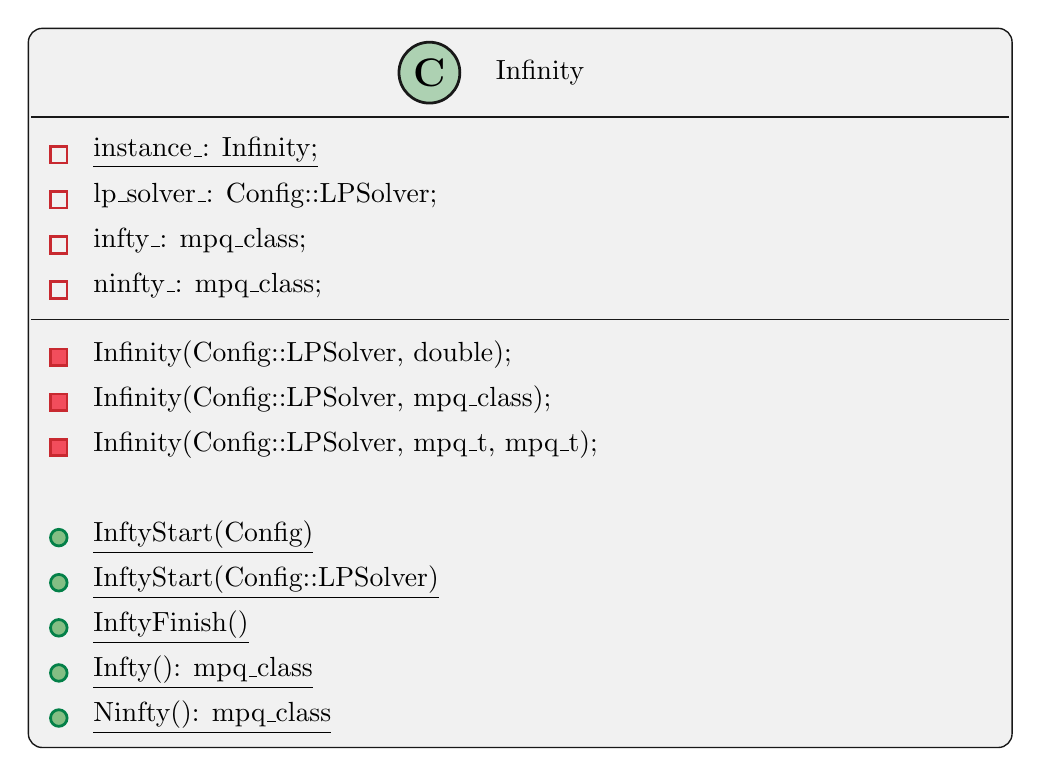
\begin{tikzpicture}[yscale=-1
,pstyle2/.style={color=plantucolor0001,line width=0.5pt}
,pstyle3/.style={color=plantucolor0004,line width=1.0pt}
,pstyle4/.style={color=plantucolor0004,fill=plantucolor0005,line width=1.0pt}
,pstyle5/.style={color=plantucolor0007,fill=plantucolor0006,line width=1.0pt}
]
\draw[color=plantucolor0001,fill=plantucolor0000,line width=0.5pt] (7pt,12pt) arc (180:270:5pt) -- (12pt,7pt) -- (357.4621pt,7pt) arc (270:360:5pt) -- (362.4621pt,12pt) -- (362.4621pt,261.8594pt) arc (0:90:5pt) -- (357.4621pt,266.8594pt) -- (12pt,266.8594pt) arc (90:180:5pt) -- (7pt,261.8594pt) -- cycle;
\draw[color=plantucolor0001,fill=plantucolor0002,line width=1.0pt] (151.921pt,23pt) ellipse (11pt and 11pt);
\node at (151.921pt,23pt)[]{\textbf{\Large C}};
\node at (172.421pt,14.8516pt)[below right,color=black]{Infinity};
\draw[pstyle2] (8pt,39pt) -- (361.4621pt,39pt);
\draw[pstyle3] (15pt,49.6484pt) rectangle (21pt,55.6484pt);
\node at (27pt,43pt)[below right,color=black]{\underline{instance\_: Infinity;}};
\draw[pstyle3] (15pt,65.9453pt) rectangle (21pt,71.9453pt);
\node at (27pt,59.2969pt)[below right,color=black]{lp\_solver\_: Config::LPSolver;};
\draw[pstyle3] (15pt,82.2422pt) rectangle (21pt,88.2422pt);
\node at (27pt,75.5938pt)[below right,color=black]{infty\_: mpq\_class;};
\draw[pstyle3] (15pt,98.5391pt) rectangle (21pt,104.5391pt);
\node at (27pt,91.8906pt)[below right,color=black]{ninfty\_: mpq\_class;};
\draw[pstyle2] (8pt,112.1875pt) -- (361.4621pt,112.1875pt);
\draw[pstyle4] (15pt,122.8359pt) rectangle (21pt,128.8359pt);
\node at (27pt,116.1875pt)[below right,color=black]{Infinity(Config::LPSolver, double);};
\draw[pstyle4] (15pt,139.1328pt) rectangle (21pt,145.1328pt);
\node at (27pt,132.4844pt)[below right,color=black]{Infinity(Config::LPSolver, mpq\_class);};
\draw[pstyle4] (15pt,155.4297pt) rectangle (21pt,161.4297pt);
\node at (27pt,148.7813pt)[below right,color=black]{Infinity(Config::LPSolver, mpq\_t, mpq\_t);};
\node at (27pt,165.0781pt)[below right,color=black]{ };
\draw[pstyle5] (18pt,191.0234pt) ellipse (3pt and 3pt);
\node at (27pt,181.375pt)[below right,color=black]{\underline{InftyStart(Config)}};
\draw[pstyle5] (18pt,207.3203pt) ellipse (3pt and 3pt);
\node at (27pt,197.6719pt)[below right,color=black]{\underline{InftyStart(Config::LPSolver)}};
\draw[pstyle5] (18pt,223.6172pt) ellipse (3pt and 3pt);
\node at (27pt,213.9688pt)[below right,color=black]{\underline{InftyFinish()}};
\draw[pstyle5] (18pt,239.9141pt) ellipse (3pt and 3pt);
\node at (27pt,230.2656pt)[below right,color=black]{\underline{Infty(): mpq\_class}};
\draw[pstyle5] (18pt,256.2109pt) ellipse (3pt and 3pt);
\node at (27pt,246.5625pt)[below right,color=black]{\underline{Ninfty(): mpq\_class}};
\end{tikzpicture}
